% Copyright (C) 2012 Shi.Zhan <g.shizhan.g@gmail.com>
%
% Permission is hereby granted, free of charge, to any person obtaining a copy of this software and associated documentation files (the "Software"), to deal in the Software without restriction, including without limitation the rights to use, copy, modify, merge, publish, distribute, sublicense, and/or sell copies of the Software, and to permit persons to whom the Software is furnished to do so, subject to the following conditions:
%
% The above copyright notice and this permission notice shall be included in all copies or substantial portions of the Software.
%
% THE SOFTWARE IS PROVIDED "AS IS", WITHOUT WARRANTY OF ANY KIND, EXPRESS OR IMPLIED, INCLUDING BUT NOT LIMITED TO THE WARRANTIES OF MERCHANTABILITY, FITNESS FOR A PARTICULAR PURPOSE AND NONINFRINGEMENT. IN NO EVENT SHALL THE AUTHORS OR COPYRIGHT HOLDERS BE LIABLE FOR ANY CLAIM, DAMAGES OR OTHER LIABILITY, WHETHER IN AN ACTION OF CONTRACT, TORT OR OTHERWISE, ARISING FROM, OUT OF OR IN CONNECTION WITH THE SOFTWARE OR THE USE OR OTHER DEALINGS IN THE SOFTWARE.
%
% 课程:人机交互技术及应用
% 班级:传播学1001班
% 课时:40学时,2012年秋季1~10周,每周一、三
% 地点:东九楼D212
% 主页:http://code.google.com/p/hci-course/
% 教师:施展 
% 单位:华中科技大学 武汉光电国家实验室
%
\documentclass{beamer}
\usepackage{fontspec,xunicode,xltxtra,beamerthemesplit}
%\usetheme{Hannover} % White background
\usetheme{Berkeley} % Blue background
\setsansfont[Mapping=tex-text, ItalicFont={Courier Italic}]{Microsoft YaHei}

% 中文环境自动换行
\XeTeXlinebreaklocale "zh"
\XeTeXlinebreakskip = 0pt plus 1pt

% 中文环境修正导航栏
\makeatletter
\def\beamer@linkspace#1{%
  \begin{pgfpicture}{0pt}{-1.5pt}{#1}{5.5pt}
    \pgfsetfillopacity{0}
    \pgftext[x=0pt,y=-1.5pt]{.}
    \pgftext[x=#1,y=5.5pt]{.}
  \end{pgfpicture}}
\makeatother

% diagrams
\usepackage{tikz}

\title{人机交互技术}
\author{施展}
\institute{华中科技大学~武汉光电国家实验室}
\date{\today}
\titlegraphic{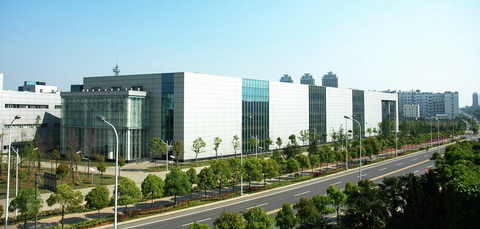
\includegraphics[width=3.5cm]{images/wnlo.jpg}}

\begin{document}

\begin{frame}
	\titlepage
\end{frame}

\begin{frame}
	\frametitle{内容提要}
	\tableofcontents
\end{frame}

\section{第二讲}
\begin{frame}
	\frametitle{第二讲 感知和认知基础}
	\begin{itemize}
		\item 人的感知
		\item 认知过程与交互设计原则
		\item 概念模型及认知
		\item 分布式认知
	\end{itemize}
\end{frame}

\subsection{人的感知}
\begin{frame}
	\frametitle{人的感知}
	\beamertemplatetransparentcovereddynamicmedium 
	\begin{itemize}[<+->]
		\item 人的感知即\textbf{通过人体器官和组织进行人与外部世界的信息的交流和传递}
		\item 认知是人们在进行日常活动时发生于头脑中的事情
		\begin{itemize}
			\item 涉及思维、记忆、学习、幻想、决策、看、读、写和交谈等
		\end{itemize}
		\item 人的感知是认知的基础,认知是将感知获取的信息综合运用
		\begin{itemize}
			\item 认知分为\textbf{经验认知}和\textbf{思维认知}
			\item 认知过程是相互联系的,单纯的一个认知过程是非常少见的
		\end{itemize}
	\end{itemize}
\end{frame}

\begin{frame}
	\frametitle{认知心理学 Cognitive Psychology}
	\beamertemplatetransparentcovereddynamicmedium 
	\begin{itemize}
		\item 认知心理学是二十世纪50年代中期在西方兴起的一种心理学思潮,二十世纪70年代开始其成为西方心理学的一个主要研究方向。\pause
		\item 是构成人类行为基础的心理机制,其核心是输入和输出之间发生的内部心理过程。\pause
		\item 与西方传统哲学也有一定联系,其主要特点是\textbf{强调知识的作用,认为知识是决定人类行为的主要因素}。\pause
		\item 认知心理学研究:
		\begin{itemize}
			\item 人们如何获得外部世界信息
			\item 信息在人脑内如何表示并转化为知识
			\item 知识怎样存储又如何用来指导人们的注意和行为
		\end{itemize}
	\end{itemize}
\end{frame}

\begin{frame}
	\frametitle{感知通道}
	\beamertemplatetransparentcovereddynamicmedium 
	\begin{itemize}
		\item \onslide<1->{五种基本感知的绝对阈限:}
		\begin{itemize}
			\item \textbf{视觉}: \onslide<2->{在黑暗而空气清新的夜晚, 人们可以看到48公里外的一只烛光;} 
			\item \textbf{听觉}: \onslide<3->{在安静的环境中, 人能够听到6米远处的手表滴答声;}
			\item \textbf{嗅觉}: \onslide<4->{人能嗅到1公升空气中散布的1/10万毫克的人造麝香的气味; }
			\item \textbf{味觉}: \onslide<5->{人可尝出9升水中放一茶匙糖的甜味; }
			\item \textbf{触觉}: \onslide<6->{人可感到蜂蜜翅膀距脸颊1厘米处落下。}
		\end{itemize}
	\end{itemize}
\end{frame}

\begin{frame}
	\frametitle{视觉感知}
	\beamertemplatetransparentcovereddynamicmedium 
	\begin{itemize}[<+->]
		\item 外界\textbf{80\%的信息}都是通过视觉得到的,视觉是人与周围世界发生联系的最重要的感觉通道。
		\item 视觉显示是人机交互系统中用的最多的人机界面。
		\item 视觉感知两阶段:\textbf{受到外部刺激接收信息阶段}和\textbf{解释信息阶段}。
	\end{itemize}	
\end{frame}

\begin{frame}
	\frametitle{视觉感知~{\small 特点}}
	\beamertemplatetransparentcovereddynamicmedium
	\transwipe
	\setbeamercolor{uppercol}{fg=white,bg=green!80!gray}
	\setbeamercolor{lowercol}{fg=black,bg=green!20!white}
	\begin{columns}
		\column{5cm}
		\onslide<1->{
			\begin{beamerboxesrounded}[upper=uppercol,lower=lowercol,shadow=true]{受到外部刺激接收信息}
				眼睛和视觉系统的物理特性决定了人类无法看到某些事物
			\end{beamerboxesrounded}
		}
		\column{5cm}
		\onslide<2->{
			\begin{beamerboxesrounded}[upper=uppercol,lower=lowercol,shadow=true]{解释信息}
				视觉系统进行解释处理信息时可对不完全信息发挥一定的想象力
			\end{beamerboxesrounded}
		}
	\end{columns}
	~\\
	\onslide<3->{进行人机交互设计需要清楚这两个阶段及其影响,了解人类真正能够看到的信息。}
\end{frame}

\begin{frame}
	\frametitle{眼睛的构造}
	\transboxout
	\begin{center}
		\only<1>{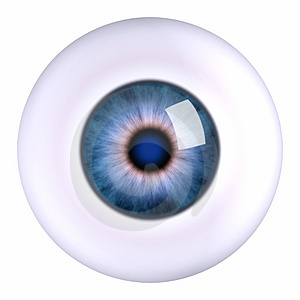
\includegraphics[width=7cm]{images/eyeball.jpg}}
		\only<2>{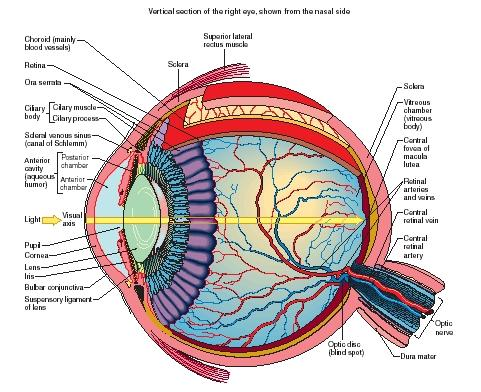
\includegraphics[width=8cm]{images/eyeball-anatomy.jpg}}
	\end{center}
\end{frame}

\begin{frame}
	\frametitle{视干细胞和视锥细胞}
	\begin{tabular}[t]{p{4.5cm}|p{4.5cm}}
		\hline
		视干细胞 & 视锥细胞\\	\hline
		在低水平照明时起作用 & 在高水平照明时起作用\\\hline
		区别黑白 & 区别彩色\\	\hline
		对光谱中绿色部分最敏感 & 对光谱中黄色部分最敏感\\\hline
		在远离视网膜中心处最多 & 在视网膜中部最多\\\hline
		对极弱的刺激敏感 & 识别空间位置、敏锐地看物体\\\hline
	\end{tabular}
\end{frame}

\begin{frame}
	\frametitle{视角和视敏度}
	\beamertemplatetransparentcovereddynamicmedium
	\begin{columns}
		\column{7.5cm}
		\begin{center}
			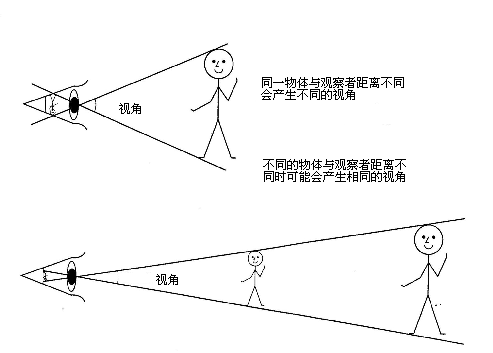
\includegraphics[width=5cm]{images/viewport.png}
		\end{center}
		\begin{itemize}[<+->]
			\item 视敏度:{\tiny 指人眼对细节的感知能力,通常用被辨别物体最小间距所对应的视角的倒数表示。通常将能分辨出视角1′的视敏度定为1.0。}
			\item 一般人能够在2m的距离分辨2mm-20mm的间距,为我们设计界面时字符大小和间距提供了依据
		\end{itemize}
	\column{2.5cm}
	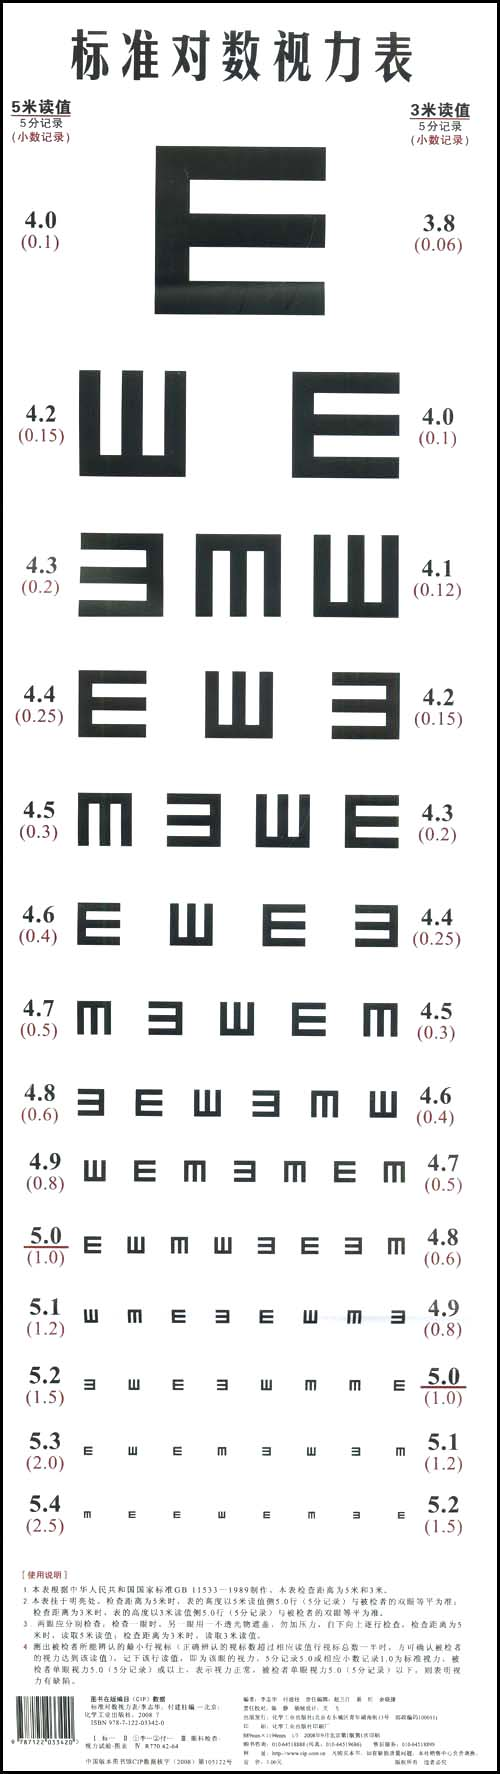
\includegraphics[width=2cm]{images/eye-chart.jpg}
	\end{columns}
\end{frame}

\begin{frame}
	\frametitle{感知物体大小、相对距离和深度}
	\beamertemplatetransparentcovereddynamicmedium
	\begin{columns}
	\column{5cm}
	利用视觉影像中的线索:
	\begin{itemize}
		\item<1-> 覆盖关系\\{\tiny 被覆盖的物体相对较远;}
		\item<2-> 大小比例\\{\tiny 一般来讲,较大的物体距离较近;}
		\item<3-> 对物体的熟悉度\\{\tiny 对非常熟悉物体,人们对物体的大小在头脑中事先有一个期望和预测,因此在判断物体距离时很容易和他看到的物体的大小联系起来。} 
	\end{itemize}
	\column{5cm}
	\begin{center}
		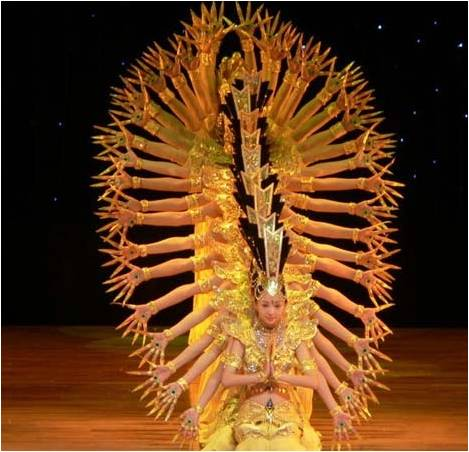
\includegraphics[width=4cm]{images/depth.jpg}
	\end{center}
	\end{columns}
\end{frame}

\begin{frame}
	\frametitle{感知亮度及色彩}
	\beamertemplatetransparentcovereddynamicmedium
	\begin{center}
		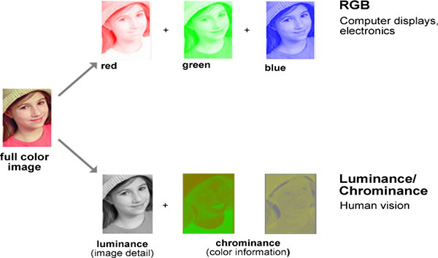
\includegraphics[width=6cm]{images/04_rgb_luminance.jpg}
	\end{center}
%	\begin{itemize}
%		\item 亮度是光线明亮程度的主观反映 
%		\item 增强亮度可以提高视敏度 
%		\item 随着亮度的增加,闪烁感也会增强。~在高亮度时,光线变化低于50Hz,视觉系统就会感到闪烁
%	\end{itemize}
%	\begin{itemize}
%		\item 人能感觉到不同的颜色,这是眼睛接受不同波长的光的结果。 
%		\item 颜色通常用三种属性表示:色度、强度和饱和度。
%		\item 色度是由光的波长决定的,正常的眼睛可感受到的光谱波长为400μm-700μm。
%	\end{itemize}
	\begin{itemize}[<+->]
		\item 视敏度影响、闪烁感与50Hz界限
		\item 波长,可视光谱,三种属性:\\{\tiny 色度 chrominance、强度 luminance 和饱和度 saturation}
		\item 在设计交互界面时,要\textbf{考虑使用者对亮度、闪烁以及色彩对比的感知},避免疲劳,创造舒适的交互环境。
	\end{itemize}
\end{frame}

\begin{frame}
	\frametitle{视觉行为的整体性}
	格式塔 (Gestalt) 心理学\\
	\begin{center}
	\begin{tikzpicture}
		\onslide<1>{
			\foreach \c in {(1,0), (0,1), (2,1), (1,2)} \fill \c + (0.5,0.5) circle (0.50);
			\foreach \c in {(6,0), (5,1), (7,1), (6,2)} \fill \c + (0.5,0.5) circle (0.30);
		}
		\onslide<1,2>{
			\foreach \c in {(1,1)} \fill \c + (0.5,0.5) circle (0.40);
			\foreach \c in {(6,1)} \fill \c + (0.5,0.5) circle (0.40);
		}
	\end{tikzpicture}
	\end{center}
\end{frame}

\begin{frame}
	\frametitle{视觉行为的整体性}
	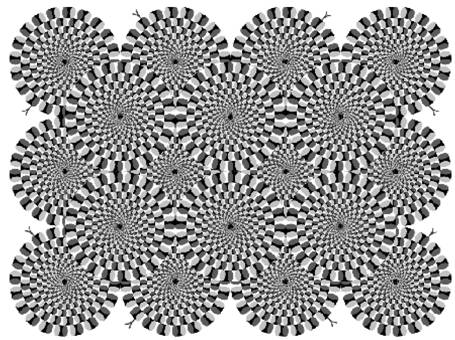
\includegraphics[width=9cm]{images/gestalt1.jpg}
\end{frame}

\subsection{认知过程与交互设计原则}
\begin{frame}
	\frametitle{认知过程与交互设计原则}

\end{frame}

\subsection{概念模型及认知}
\begin{frame}
	\frametitle{概念模型及认知}
	\begin{center}
		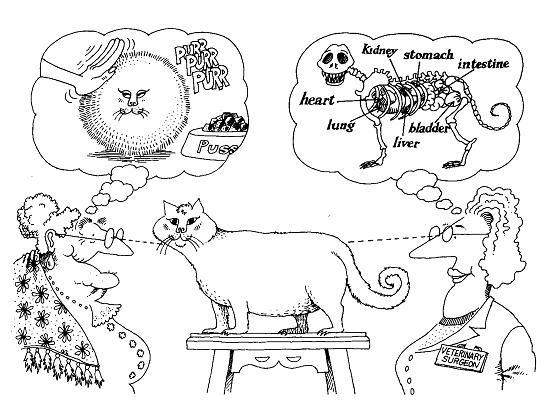
\includegraphics[width=8cm]{images/viewpoint.jpg}
	\end{center}
\end{frame}

\subsection{分布式认知}
\begin{frame}
	\frametitle{分布式认知}

\end{frame}

\begin{frame}
	\frametitle{分布式认知模型}
	\beamertemplatetransparentcovereddynamicmedium
	\begin{itemize}
		\item 分布式认知法描述的是认知系统中发生了什么,它通常描述人员之间的交互,人们使用的物品及工作环境。\pause
		\item 例如,要驾驶飞机这个活动涉及:
		\begin{itemize}
			\item 驾驶员、副驾驶员和空中交通管制员之间的交互;
			\item 驾驶员、副驾驶员与驾驶舱内各种仪表的交互;
			\item 驾驶员、副驾驶员与飞机所处环境的交互,如空中航线、跑道。
		\end{itemize}\pause
		\item 分布式认知的主要目的是要从信息传播媒介的角度来描述交互。
		\begin{itemize}
			\item 信息如何表示,信息在流经不同个人以及使用不同物体时如何重新表示。
			\item 这类信息的转变也称为“表示状态的转变”。
		\end{itemize}
	\end{itemize}
\end{frame}

\begin{frame}
	\frametitle{分布式模型与传统模型}
	\transboxin<2>
	\only<1>{
		\begin{itemize}
			\item Hollan, Hutchins \& Kirsh (2000) observing human activity ``in the wild,'' described three ways that cognitive process can be distributed
			\begin{enumerate}
				\item They can be distributed across members of a social group either co-present or over a distance.
				\item They can distributed between internal process and external (material or environmental) tools.
				\item They can be distributed across time with products of earlier events transforming the nature of later events.
			\end{enumerate}
		\end{itemize}
    	\begin{flushright}
    		{\tiny http://mindmaps.wikispaces.com/dcog}
    	\end{flushright}
	}
	\only<2>{
		\begin{center}
			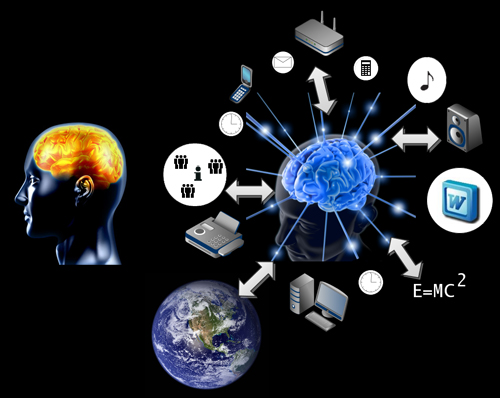
\includegraphics[width=8cm]{images/cognition4.jpg}
		\end{center}
	}
\end{frame}

\begin{frame}
	\frametitle{分布式认知模型}
	\beamertemplatetransparentcovereddynamicmedium
	\begin{itemize}
		\item 在进行分布式认知分析时,通常需要考查:\pause
		\begin{itemize}
			\item 分布式问题的解决方法\\{\tiny 包括协议解决方式}\pause
			\item 语言及非语言行为的任务\\{\tiny 包括说了什么、眼神和眨眼等暗示什么、什么是没有说出来的}\pause
			\item 使用的各种协调机制\\{\tiny 如规则、规程}\pause
			\item 协作活动在进行过程中将用到的各种通信路径\pause
			\item 如何共享和访问信息
		\end{itemize}
	\end{itemize}
\end{frame}

\section{小结}
\begin{frame}
	\frametitle{小结}
	\begin{itemize}
		\item 了解人的感知模型
		\item 掌握认知过程与交互设计原则
		\item 掌握概念模型及对概念模型的认知
		\item 了解分布式认知
	\end{itemize}
\end{frame}
 
\end{document}